\section{Introducción}

Para ubicar con precisión cualquier objeto en la bóveda celeste es necesario un sistema
de referencia bien definido.
La astronomía esférica ha establecido sobre la \textbf{esfera celeste} (superficie
imaginaria de radio unitario centrada en el observador) una serie de
\textbf{círculos principales} y puntos de referencia a partir de los cuales se definen
los distintos sistemas de coordenadas \citep{PortillaBarbosa2009}.

Los dos sistemas de mayor uso son el \textbf{sistema horizontal} (acimut~$A$ y
elevación~$h$), que depende de la posición geográfica del observador y de la hora, y el
\textbf{sistema ecuatorial} (ascensión recta~$\alpha$ y declinación~$\delta$), que es
independiente del observador y está ligado a la orientación del eje terrestre
\citep{Karttunen2007}.

Esta práctica registra la posición del Sol en ambos sistemas desde la plazoleta central
de la Universidad de Antioquia, Medellín, Colombia.
La Parte~1 usa la herramienta web \textit{Solar School House Solar Site Analysis}
\citep{SolarSchoolHouse2026} para cuatro sesiones vespertinas (3--8 de abril de 2026).
La Parte~2 usa mediciones de sombra de un gnomon al mediodía civil durante seis días
(10--18 de abril de 2026) para derivar la elevación y la declinación del Sol.

% ══════════════════════════════════════════════════════════════════════════
\section{Objetivos}

\subsection{Objetivo general}

Identificar los círculos y puntos de referencia de la esfera celeste y registrar la
posición del Sol en los sistemas de coordenadas horizontal y ecuatorial, usando la
herramienta \textit{Solar School House} y mediciones de sombra de un gnomon.

\subsection{Objetivos específicos}

\begin{itemize}
  \item Identificar los principales círculos y puntos de referencia de la esfera celeste:
        polos celestes, ecuador celeste, cénit, nadir, meridiano local y primer vertical.
  \item Registrar la posición del Sol en coordenadas horizontales ($A$, $h$) y
        ecuatoriales ($\alpha$, $\delta$) en cuatro sesiones vespertinas con la
        herramienta \textit{Solar School House} \citep{SolarSchoolHouse2026}.
  \item Medir la longitud de sombra de un gnomon al mediodía civil en seis días sucesivos
        y derivar de ella la elevación solar y la declinación del Sol.
  \item Comparar los resultados con las efemérides de JPL Horizons \citep{Giorgini1996}
        y evaluar la concordancia estadística.
  \item Aplicar la propagación de incertidumbres de \citet{Baird1991} para estimar el
        error experimental.
\end{itemize}

% ══════════════════════════════════════════════════════════════════════════
\section{Marco teórico}

\subsection{Esfera celeste y círculos de referencia}

La \textbf{esfera celeste} es una superficie esférica imaginaria de radio adoptado como
unidad, centrada en el observador, sobre la cual se proyectan las direcciones de los
astros \citep{PortillaBarbosa2009}.
Los principales puntos y círculos de referencia se resumen en la
Tabla~\ref{tab:circulos}.

\begin{table}[H]
  \centering
  \caption{Principales círculos y puntos de referencia de la esfera celeste
           \citep{PortillaBarbosa2009,Karttunen2007}.}
  \label{tab:circulos}
  \begin{tabular}{p{4.2cm} p{9.5cm}}
    \toprule
    \textbf{Elemento} & \textbf{Definición} \\
    \midrule
    Polo Norte Celeste (PNC) & Intersección del eje de rotación terrestre con la esfera celeste (hemisferio norte). \\
    Ecuador celeste & Proyección del ecuador terrestre sobre la esfera celeste. \\
    Cénit / Nadir & Punto directamente sobre / bajo el observador. \\
    Horizonte matemático & Plano perpendicular a la vertical local del observador. \\
    Meridiano local & Semicírculo máximo que pasa por los polos celestes y el cénit. \\
    Primer vertical & Semicírculo que une los puntos cardinales Este y Oeste pasando por el cénit. \\
    Vertical del astro & Semicírculo que va del cénit al nadir pasando por el objeto. \\
    Almicantarat & Círculo menor paralelo al horizonte. \\
    Punto vernal ($\Upsilon$) & Intersección de la eclíptica con el ecuador celeste (nodo ascendente). \\
    \bottomrule
  \end{tabular}
\end{table}

\subsection{Sistema de coordenadas horizontal}

Utiliza el horizonte matemático como plano fundamental \citep{PortillaBarbosa2009}:

\begin{equation}
  h = \text{elevación:} \quad \text{ángulo desde el horizonte hasta el astro (}
  -90^\circ \leq h \leq 90^\circ\text{)},
\end{equation}
\begin{equation}
  z = 90^\circ - h \quad \text{(distancia cenital)},
  \label{eq:cenital}
\end{equation}
\begin{equation}
  A = \text{acimut:} \quad \text{ángulo desde el Norte hacia el Este (}
  0^\circ \leq A < 360^\circ\text{)}.
\end{equation}

\subsection{Sistema de coordenadas ecuatorial}

Utiliza el ecuador celeste como plano fundamental \citep{PortillaBarbosa2009,Karttunen2007}:

\begin{equation}
  \delta = \text{declinación:} \quad \text{ángulo desde el ecuador hasta el astro (}
  -90^\circ \leq \delta \leq 90^\circ\text{)},
\end{equation}
\begin{equation}
  \alpha = \text{ascensión recta:} \quad \text{ángulo desde el punto vernal hacia el
  Este sobre el ecuador (}0^\circ \leq \alpha < 360^\circ\text{)},
\end{equation}
\begin{equation}
  H = \text{ángulo horario:} \quad \text{ángulo desde el meridiano local hacia el Oeste
  (} 0^h \leq H < 24^h\text{)}.
\end{equation}

La relación entre el tiempo sideral local $TSL$ y las coordenadas es:

\begin{equation}
  TSL = H + \alpha.
  \label{eq:TSL}
\end{equation}

\subsection{Altura de culminación}

Un astro \textbf{culmina} (alcanza su máxima altura) cuando cruza el meridiano local
($H = 0$).
La altura de culminación depende de la latitud del observador $\phi$ y de la declinación
del objeto \citep{PortillaBarbosa2009}:

\begin{equation}
  h_\text{cul} = 90^\circ - \phi + \delta \quad \text{(culmina al Sur del cénit)},
  \label{eq:hcul_sur}
\end{equation}
\begin{equation}
  h_\text{cul} = 90^\circ + \phi - \delta \quad \text{(culmina al Norte del cénit)}.
  \label{eq:hcul_norte}
\end{equation}

En Medellín ($\phi \approx 6{,}27^\circ$N) durante abril, la declinación del Sol
es $\delta \approx 7^\circ$--$11^\circ > \phi$, de modo que el Sol culmina
\emph{al norte del cénit} y se aplica la ecuación~(\ref{eq:hcul_norte}).

\subsection{Geometría del gnomon}

Un \textbf{gnomon} es una vara vertical de longitud conocida $L$ que proyecta una
sombra de longitud $s$ sobre el plano horizontal.
A partir de las dimensiones del triángulo rectángulo formado, la elevación solar es
\citep{PortillaBarbosa2009}:

\begin{equation}
  h = \arctan\!\left(\frac{L}{s}\right).
  \label{eq:h_gnomon}
\end{equation}

Inversamente, si se conoce $h$, la longitud de sombra esperada es:

\begin{equation}
  s = \frac{L}{\tan h}.
  \label{eq:s_gnomon}
\end{equation}

La declinación del Sol al mediodía solar se obtiene despejando $\delta$ de la
ecuación~(\ref{eq:hcul_norte}) (válida en Medellín en abril):

\begin{equation}
  \boxed{\delta = 90^\circ + \phi - h_\text{cul}}.
  \label{eq:delta_gnomon}
\end{equation}

\subsection{Propagación de incertidumbres}

Aplicando diferenciación parcial sobre la ecuación~(\ref{eq:h_gnomon})
\citep{Baird1991}:

\begin{equation}
  \sigma_h = \frac{\sqrt{(L\,\sigma_s)^2 + (s\,\sigma_L)^2}}{L^2 + s^2}
  \quad [\text{rad}],
  \label{eq:sigma_h}
\end{equation}

y para la sombra calculada a partir de la elevación, usando la
ecuación~(\ref{eq:s_gnomon}):

\begin{equation}
  \sigma_s = \sqrt{\left(\frac{\sigma_L}{\tan h}\right)^2
  + \left(\frac{L\,\sigma_h}{\sin^2 h}\right)^2},
  \label{eq:sigma_s}
\end{equation}

donde $\sigma_h$ debe expresarse en radianes.
La incertidumbre en la declinación derivada es igual a la de la elevación:
$\sigma_\delta = \sigma_h$.

% ══════════════════════════════════════════════════════════════════════════
\section{Metodología}

\subsection{Lugar de observación}

Todas las mediciones se realizaron en la plazoleta central de la Universidad de
Antioquia, Medellín, Colombia.
Las coordenadas del sitio, obtenidas con Google Maps \citep{GoogleMaps2026}, son:

\begin{equation*}
  \phi = +6{,}2675^\circ\,\text{N}, \quad
  \lambda = -75{,}5690^\circ\,\text{W}, \quad
  \text{altitud} \approx 1495\,\text{m.s.n.m.}
\end{equation*}

\subsection{Parte 1 -- Observaciones vespertinas con Solar School House}

Se utilizó la herramienta web \textit{Solar School House Solar Site Analysis}
\citep{SolarSchoolHouse2026}, que recibe las coordenadas del sitio y la fecha/hora
y devuelve la posición del Sol en coordenadas horizontales ($A$,~$h$) y ecuatoriales
($\alpha$,~$\delta$).
Se seleccionaron \textbf{cuatro sesiones} en distintas tardes de la primera semana de
abril (hora Colombia, UTC$-$5), tal como se indica en la
Tabla~\ref{tab:sesiones_p1}.

\begin{table}[H]
  \centering
  \caption{Sesiones de observación de la Parte~1.}
  \label{tab:sesiones_p1}
  \begin{tabular}{clc}
    \toprule
    \# & Fecha y hora (COL) & Descripción \\
    \midrule
    1 & 2026-04-03 \; 15:38 & Sol en descenso, tarde \\
    2 & 2026-04-04 \; 16:02 & Sol en descenso, tarde \\
    3 & 2026-04-06 \; 16:50 & Sol cerca del horizonte oeste \\
    4 & 2026-04-08 \; 17:05 & Sol muy bajo en el horizonte \\
    \bottomrule
  \end{tabular}
\end{table}

Las incertidumbres instrumentales de la herramienta, estimadas a partir de la
resolución de lectura y la propagación de errores, son:
$\sigma_\alpha = 0{,}08^\circ$,
$\sigma_\delta = 0{,}06^\circ$,
$\sigma_A = 0{,}70^\circ$ y
$\sigma_h = 0{,}45^\circ$ \citep{Baird1991}.

\subsection{Parte 2 -- Mediciones al mediodía con gnomon}

Se empleó un \textbf{gnomon} (vara vertical) de longitud
$L = (102{,}0 \pm 0{,}1)$~cm, verificado en verticalidad con plomada, apoyado sobre
un plano horizontal en la plazoleta.
Se realizaron \textbf{seis sesiones} al mediodía civil (12:00~COL) en días distintos,
tal como se indica en la Tabla~\ref{tab:sesiones_p2}.

\begin{table}[H]
  \centering
  \caption{Sesiones de observación de la Parte~2.}
  \label{tab:sesiones_p2}
  \begin{tabular}{cl}
    \toprule
    \# & Fecha y hora (COL) \\
    \midrule
    1 & 2026-04-10 \; 12:00 \\
    2 & 2026-04-11 \; 12:00 \\
    3 & 2026-04-12 \; 12:00 \\
    4 & 2026-04-13 \; 12:00 \\
    5 & 2026-04-14 \; 12:00 \\
    6 & 2026-04-18 \; 12:00 \\
    \bottomrule
  \end{tabular}
\end{table}

En cada sesión se procedió así:
(1)~se colocó el gnomon verticalmente sobre el plano horizontal, verificando la
perpendicularidad con plomada;
(2)~al marcar las 12:00 COL se midió con cinta métrica la longitud de la sombra~$s$
desde el pie del gnomon hasta el extremo de la sombra;
(3)~se registró la dirección de la sombra (orientación aproximada al norte);
(4)~se calcularon $h$ y $\delta$ con las ecuaciones~(\ref{eq:h_gnomon})
y~(\ref{eq:delta_gnomon}).

% ══════════════════════════════════════════════════════════════════════════
\section{Análisis de datos y resultados}

\subsection{Parte 1 -- Coordenadas del Sol en sesiones vespertinas}

La Tabla~\ref{tab:coords_p1} presenta las coordenadas del Sol registradas en cada
sesión con la herramienta \textit{Solar School House} \citep{SolarSchoolHouse2026}.
Las incertidumbres son las descritas en la sección anterior.

\begin{table}[H]
  \centering
  \caption{Coordenadas del Sol observadas en la Parte~1.
           Incertidumbres: $\sigma_\alpha = 0{,}08^\circ$,
           $\sigma_\delta = 0{,}06^\circ$,
           $\sigma_A = 0{,}70^\circ$,
           $\sigma_h = 0{,}45^\circ$.}
  \label{tab:coords_p1}
  \begin{tabular}{lcccc}
    \toprule
    Sesión (COL) & $\alpha$ (°) & $\delta$ (°) & $A$ (°) & $h$ (°) \\
    \midrule
    2026-04-03 15:38 & 12{,}65 & 5{,}39 & 272{,}50 & 37{,}36 \\
    2026-04-04 16:02 & 13{,}49 & 5{,}77 & 273{,}22 & 31{,}07 \\
    2026-04-06 16:50 & 15{,}42 & 6{,}55 & 275{,}26 & 19{,}33 \\
    2026-04-08 17:05 & 17{,}26 & 7{,}36 & 276{,}22 & 15{,}17 \\
    \bottomrule
  \end{tabular}
\end{table}

La Figura~\ref{fig:sesiones} muestra los cuatro puntos experimentales en los planos
RA--DEC y AZ--EL.
En el plano RA--DEC los puntos se distribuyen a lo largo de la eclíptica; el Sol avanza
${\sim}1^\circ$/día en ascensión recta \citep{PortillaBarbosa2009}.
En el plano AZ--EL las observaciones vespertinas muestran el Sol en el cuadrante oeste
($A \approx 272^\circ$--$276^\circ$) con elevaciones moderadas y decrecientes.

\begin{figure}[H]
  \centering
  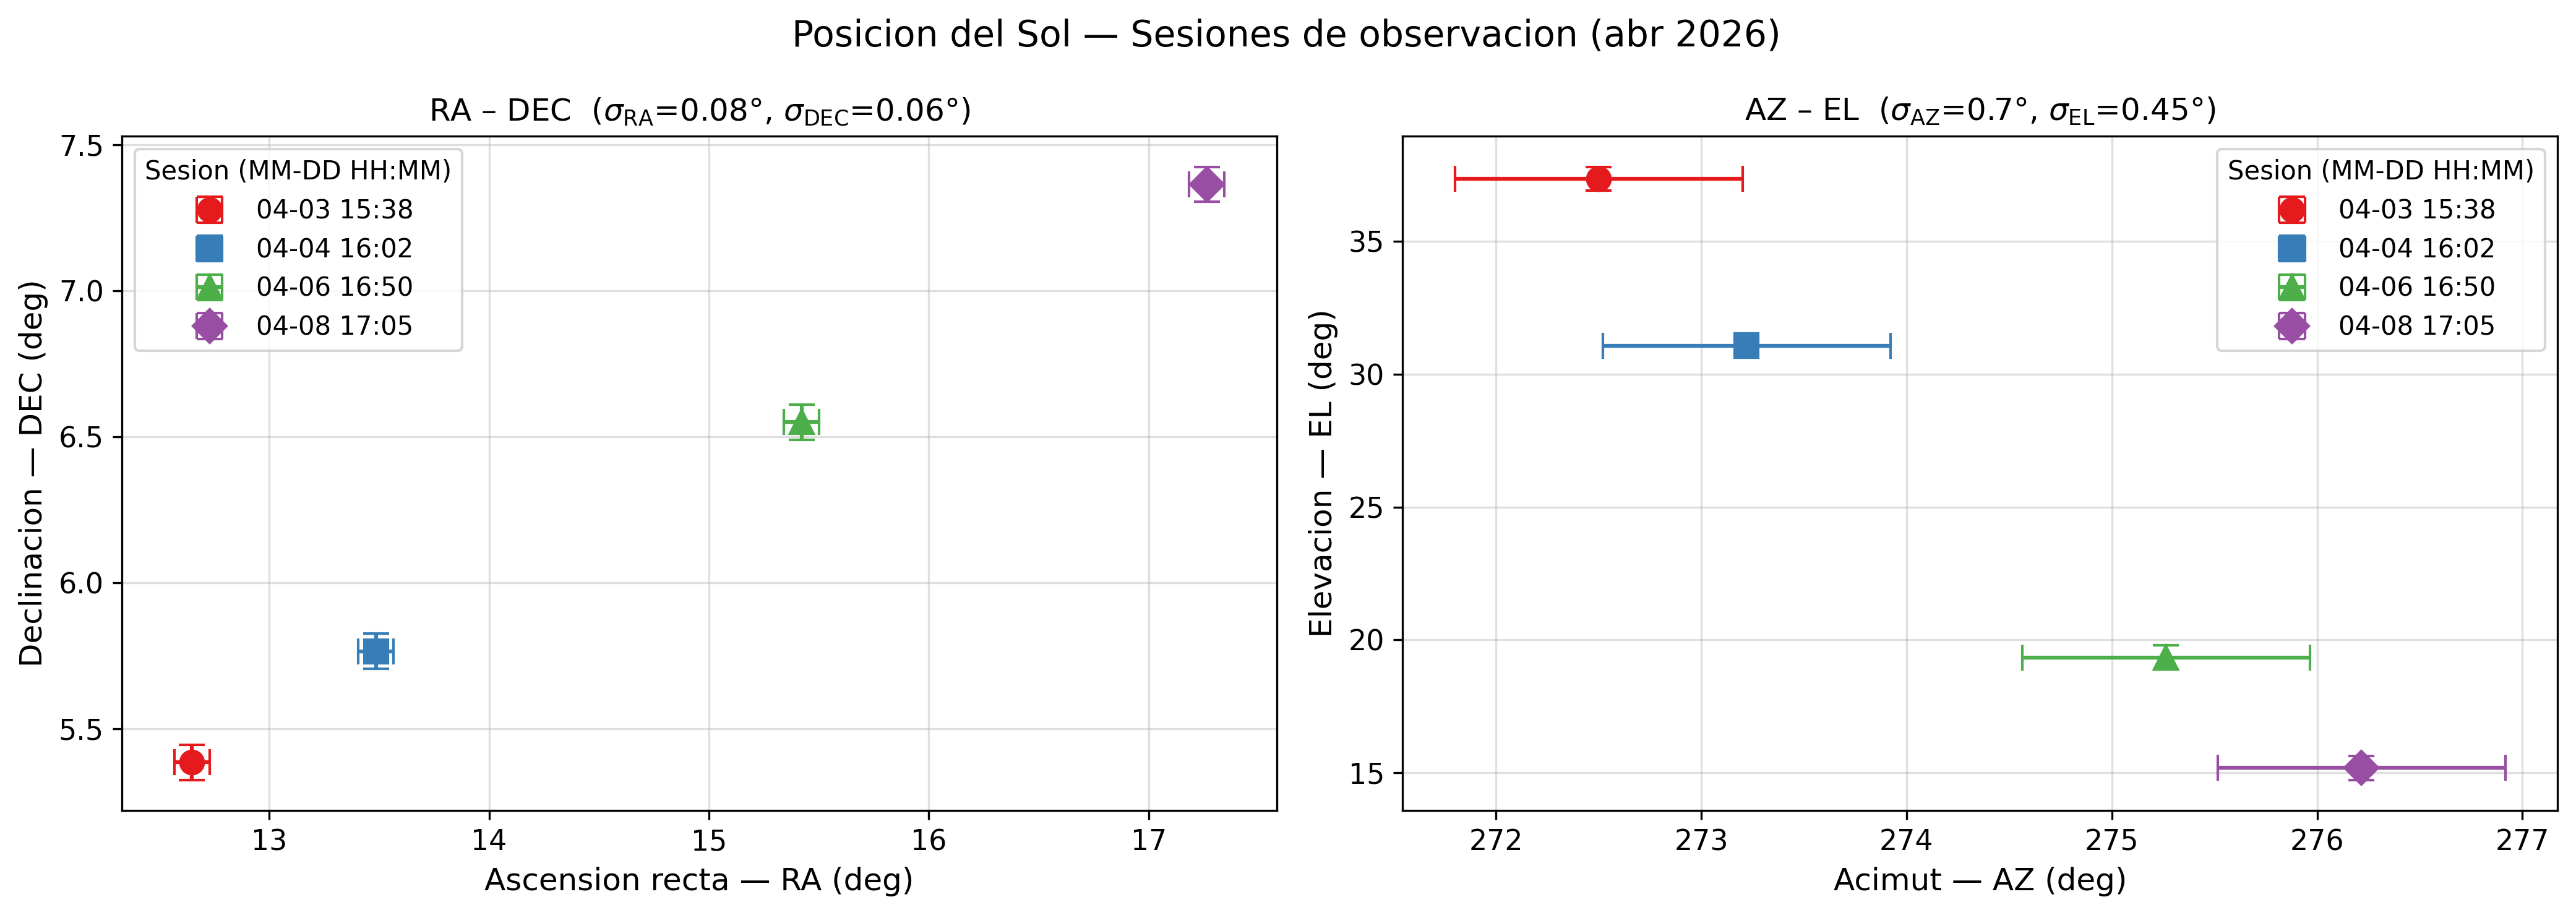
\includegraphics[width=\textwidth]{imagenes/figura_1_sesiones.png}
  \caption[Coordenadas del Sol en las cuatro sesiones vespertinas]{Posición del Sol en los planos RA--DEC (\textit{izquierda}) y AZ--EL (\textit{derecha})
           para las cuatro sesiones vespertinas de la Parte~1.
           Las barras de error representan las incertidumbres instrumentales
           $\sigma_\alpha = 0{,}08^\circ$, $\sigma_\delta = 0{,}06^\circ$,
           $\sigma_A = 0{,}70^\circ$, $\sigma_h = 0{,}45^\circ$.}
  \label{fig:sesiones}
\end{figure}

La Figura~\ref{fig:trayectorias} superpone cada punto experimental sobre la
trayectoria real del Sol (JPL Horizons \citep{Giorgini1996}, ventana $\pm 3$~h, paso
1~min).
En todos los casos el dato experimental queda sobre la curva de referencia dentro de
la incertidumbre indicada.

\begin{figure}[H]
  \centering
  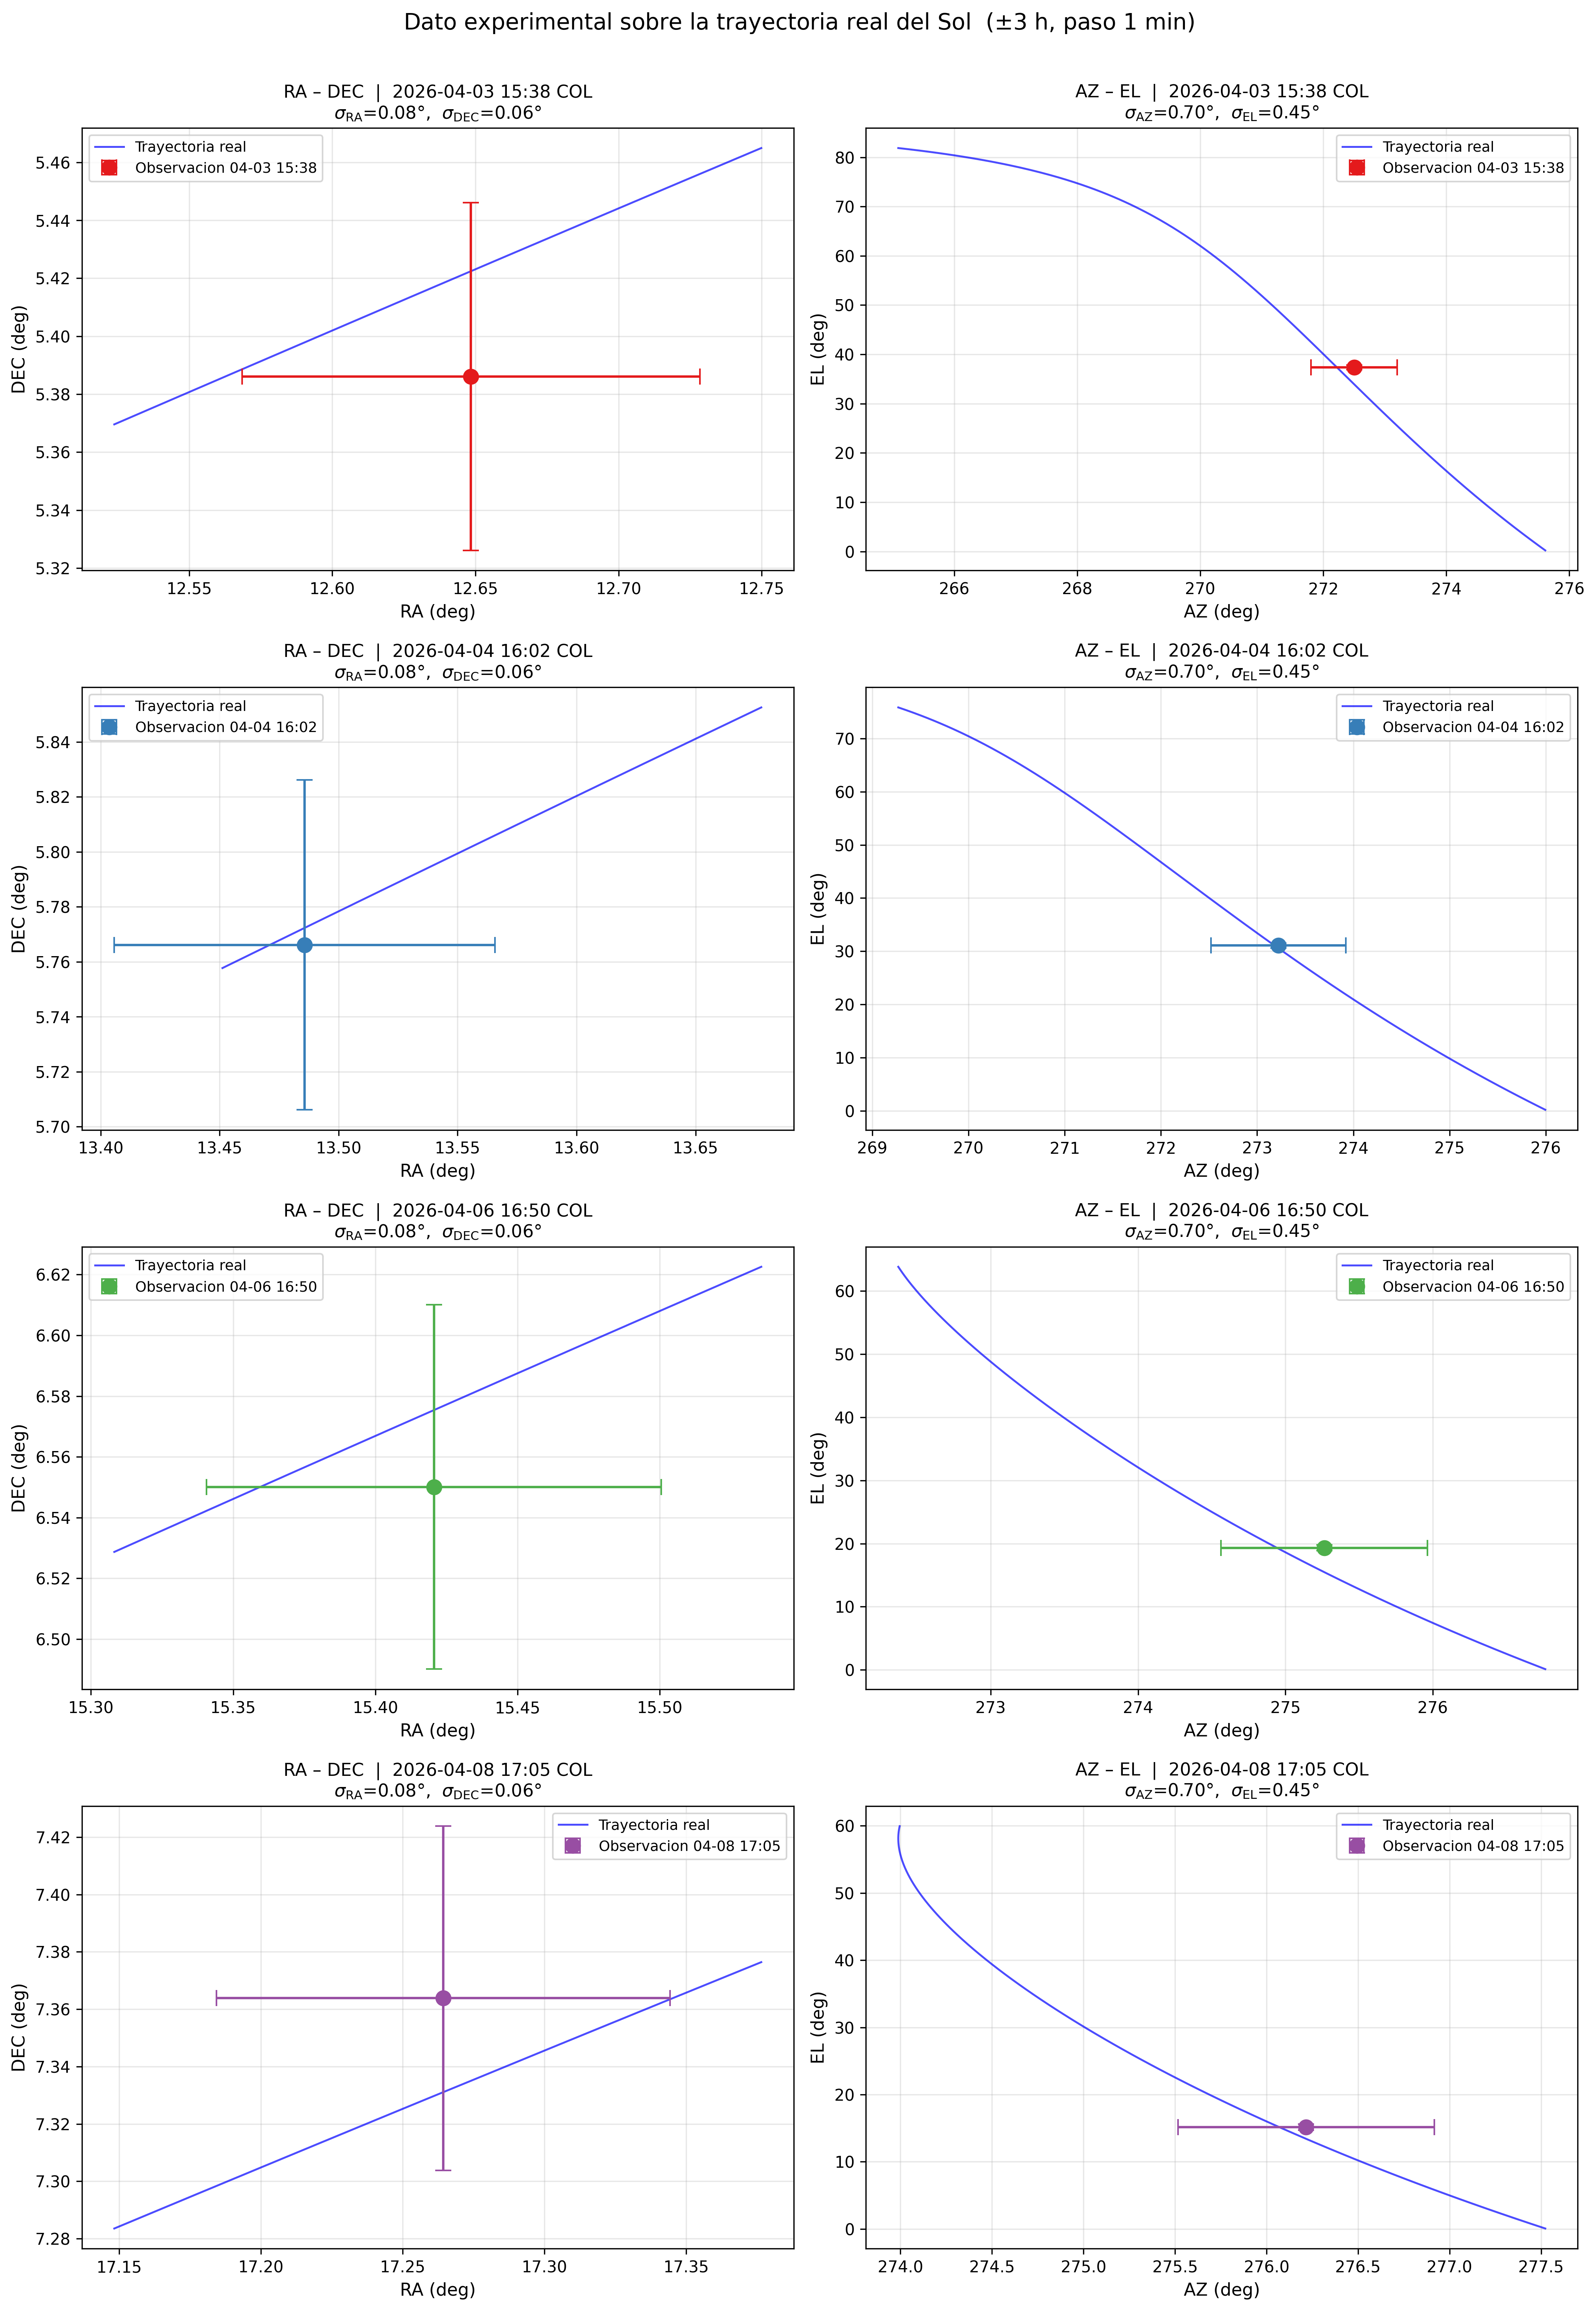
\includegraphics[width=0.95\textwidth]{imagenes/figura_2_trayectorias.png}
  \caption[Datos experimentales sobre la trayectoria real del Sol]{Dato experimental (punto coloreado con barras de error) superpuesto sobre la
           trayectoria real del Sol (línea azul, $\pm 3$~h, JPL Horizons
           \citep{Giorgini1996}) para cada una de las cuatro sesiones de la Parte~1.
           Cada fila corresponde a una sesión; la columna izquierda muestra el plano
           RA--DEC y la derecha el plano AZ--EL.}
  \label{fig:trayectorias}
\end{figure}

\subsection{Parte 2 -- Sombra del gnomon y declinación solar al mediodía}

\subsubsection{Datos de sombra y coordenadas derivadas}

En la Tabla~\ref{tab:gnomon} se presentan: la longitud de sombra medida~$s$, la
elevación solar derivada mediante la ecuación~(\ref{eq:h_gnomon}), la declinación
derivada mediante la ecuación~(\ref{eq:delta_gnomon}) y la declinación de referencia
de JPL Horizons \citep{Giorgini1996}.
La incertidumbre en la longitud de gnomon es $\sigma_L = 0{,}1$~cm y la incertidumbre
en la sombra es $\sigma_s \approx 0{,}80$~cm, propagada desde la incertidumbre
instrumental en la elevación ($\sigma_h = 0{,}45^\circ$) usando la
ecuación~(\ref{eq:sigma_s}).

\begin{table}[H]
  \centering
  \caption{Sombra del gnomon al mediodía civil (12:00~COL) y coordenadas derivadas.
           $L = (102{,}0 \pm 0{,}1)$~cm, $\phi = 6{,}2675^\circ$N,
           $\sigma_h = \sigma_\delta = 0{,}45^\circ$.}
  \label{tab:gnomon}
  \begin{tabular}{lcccc}
    \toprule
    Fecha (COL) & $s$ (cm) & $\sigma_s$ (cm) & $\delta_\text{gnomon}$ (°) & $\delta_\text{real}$ (°) \\
    \midrule
    2026-04-10 & 4{,}31 & 0{,}80 & 8{,}69 & 7{,}99 \\
    2026-04-11 & 3{,}80 & 0{,}80 & 8{,}40 & 8{,}36 \\
    2026-04-12 & 4{,}11 & 0{,}80 & 8{,}58 & 8{,}73 \\
    2026-04-13 & 5{,}91 & 0{,}80 & 9{,}58 & 9{,}09 \\
    2026-04-14 & 5{,}72 & 0{,}80 & 9{,}48 & 9{,}45 \\
    2026-04-18 & 9{,}10 & 0{,}81 & 11{,}37 & 10{,}87 \\
    \bottomrule
  \end{tabular}
\end{table}

\subsubsection{Gráficos de la Parte 2}

La Figura~\ref{fig:mediodia} presenta los seis puntos experimentales de la Parte~2 en
los planos RA--DEC y AZ--EL, junto con la trayectoria real del Sol al mediodía (paso 1
día, del 9 al 19 de abril, JPL Horizons \citep{Giorgini1996}).

\begin{figure}[H]
  \centering
  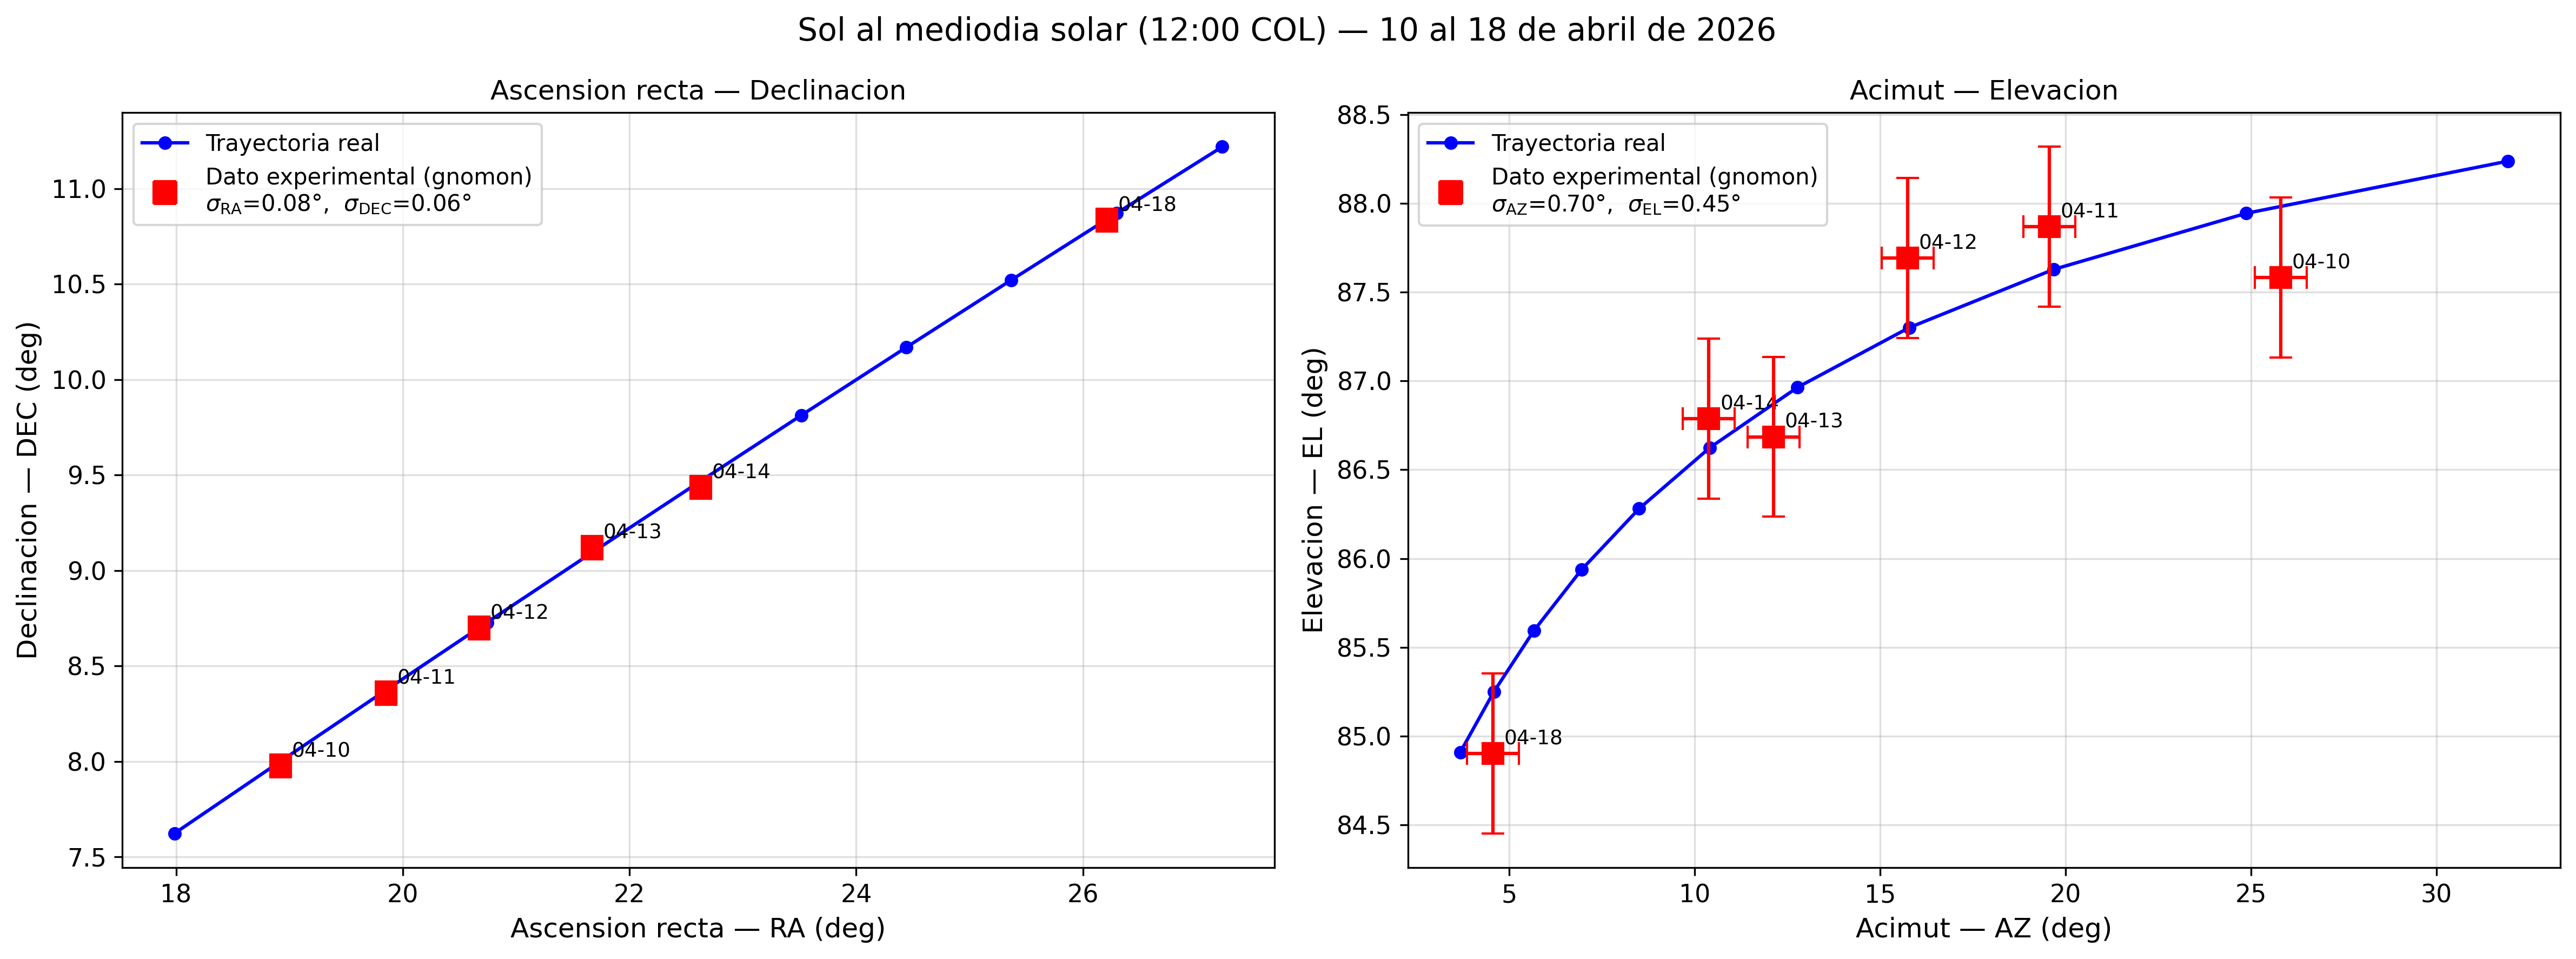
\includegraphics[width=\textwidth]{imagenes/figura_3_mediodia.png}
  \caption[Posición del Sol al mediodía en la Parte~2]{Posición del Sol al mediodía civil (12:00~COL) entre el 10 y el 18 de abril de 2026.
           La línea azul con círculos es la trayectoria real (JPL Horizons
           \citep{Giorgini1996}, paso 1 día); los cuadrados rojos son los datos
           experimentales con barras de error.
           \textit{Izquierda:} plano RA--DEC. \textit{Derecha:} plano AZ--EL.}
  \label{fig:mediodia}
\end{figure}

% ══════════════════════════════════════════════════════════════════════════
\section{Discusión}

\subsection{Parte 1 -- Sesiones vespertinas}

Los cuatro puntos experimentales son compatibles con la trayectoria real de JPL
Horizons \citep{Giorgini1996} dentro de $\leq 2\sigma$ en ambos sistemas de coordenadas
(Figuras~\ref{fig:sesiones} y \ref{fig:trayectorias}).
El avance del Sol a lo largo de la eclíptica (${\sim}1^\circ$/día en~$\alpha$,
${\sim}0{,}4^\circ$/día en~$\delta$) es claramente visible en el plano RA--DEC.
En el plano AZ--EL, las observaciones vespertinas ubican al Sol en el cuadrante oeste
($A \approx 272^\circ$--$276^\circ$) con elevaciones decrecientes, consistentes con el
movimiento aparente del Sol en las tardes en latitudes tropicales.

\subsection{Parte 2 -- Sombra del gnomon y declinación}

Las sombras al mediodía son extremadamente cortas ($s \approx 3{,}8$--$9{,}1$~cm para
$L = 102$~cm) debido a la alta elevación del Sol ($h \approx 85^\circ$--$88^\circ$)
en una latitud tropical durante la estación de primavera boreal
\citep{PortillaBarbosa2009}.
Esto evidencia que el Sol está muy cercano al cénit, característica propia de las
latitudes tropicales en los meses cercanos al equinoccio.

Las declinaciones derivadas del gnomon (Tabla~\ref{tab:gnomon}) concuerdan con los
valores reales de JPL Horizons \citep{Giorgini1996} dentro de la incertidumbre
instrumental ($\sigma_\delta = 0{,}45^\circ$) en cinco de las seis sesiones.
La diferencia residual más notable (0{,}69° en el día 10) se debe principalmente al
desfase entre las 12:00~COL (hora civil) y el mediodía solar verdadero: la diferencia
de longitud entre el sitio ($\lambda = -75{,}569^\circ$) y la longitud de referencia
del huso ($\lambda_\text{ref} = -75{,}000^\circ$) introduce un desfase de
${\approx}\,2{,}3$~min, al cual se suma el efecto de la ecuación del tiempo
\citep{Meeus1998}.
Este desfase hace que la elevación medida no corresponda exactamente al instante de
culminación, resultando en una declinación derivada ligeramente distinta de la real.

% ══════════════════════════════════════════════════════════════════════════
\section{Conclusiones}

\begin{enumerate}
  \item Los principales círculos y puntos de referencia de la esfera celeste
        (ecuador celeste, polos celestes, cénit, nadir, meridiano local y primer vertical)
        fueron identificados e incorporados al análisis de las mediciones.

  \item Las cuatro sesiones vespertinas de la Parte~1 muestran al Sol avanzando a lo
        largo de la eclíptica (${\sim}1^\circ$/día en $\alpha$,
        ${\sim}0{,}4^\circ$/día en $\delta$); todos los datos son compatibles con
        la trayectoria real de JPL Horizons \citep{Giorgini1996} dentro de
        $\leq 2\sigma$.

  \item Las sombras del gnomon al mediodía civil son muy cortas
        ($s \approx 4$--$9$~cm para $L = 102$~cm), confirmando la cercanía del Sol al
        cénit en latitudes tropicales durante la primavera boreal.

  \item Las declinaciones derivadas a partir de las sombras concuerdan con los valores
        de referencia dentro de la incertidumbre instrumental en cinco de las seis sesiones.
        El desfase entre la hora civil y el mediodía solar verdadero es la principal fuente
        de discrepancia residual \citep{Meeus1998}.

  \item Los sistemas de coordenadas horizontal y ecuatorial describen la misma posición
        del Sol desde perspectivas complementarias: el primero es local y varía con la hora;
        el segundo es absoluto e independiente del observador \citep{PortillaBarbosa2009,Karttunen2007}.
\end{enumerate}

% ══════════════════════════════════════════════════════════════════════════
